
\documentclass[xcolor=table]{beamer}

% for fancy Mike style table
 \usepackage[table]{xcolor} 
 \usepackage{multirow}
\usepackage{textpos}
\usepackage{helvet}
\usepackage{caption}
\usepackage{changepage}
\usepackage{algorithmic}
\usepackage{array}
\setbeamerfont{caption}{size = \footnotesize}
\usepackage{multicol}
\usepackage{setspace}

% useful packages for including code
\usepackage{listings}
\usepackage{color}
\lstset{breaklines}

% package for drawing graphs
\usepackage{tikz}
\usetikzlibrary{positioning}

\definecolor{charlesBlue}{RGB}{100, 155, 255}
\definecolor{charlesBlue2}{RGB}{0, 155, 255}
\definecolor{MRGGreen}{rgb}{0, 0.350, 0.200}
\usecolortheme{default}

% References
%\bibliographystyle{apacite} 
\hypersetup{colorlinks = true, linkcolor={MRGGreen}, citecolor = black, urlcolor = blue}


% Custom colors for alerts and examples
\setbeamercolor{palette primary}{fg=MRGGreen}
\setbeamercolor{palette secondary}{fg=MRGGreen}
\setbeamercolor{palette tertiary}{bg= MRGGreen}
\setbeamercolor*{structure}{fg=MRGGreen}
\setbeamercolor{titlelike}{fg=black}

\lstset{
  basicstyle=\tiny \ttfamily,
  columns=fullflexible,
}


\begin{document} 

\begin{frame}
  \begin{center}
    {\Large II} \\ \ \\ Models in pharmacometrics
  \end{center}
\end{frame}

\begin{frame}
  What is the effect of a treatment on a patient?
  \begin{itemize}
    \item \textit{pharmacokinetics (PK)}: how is the drug absorbed in the body?
    \item \textit{pharmacodynamics (PD)}: once it is absorbed, what are its effects? 
  \end{itemize}
\end{frame}

\begin{frame}
  \frametitle{Example: Two compartment model}
  
  \begin{center}
    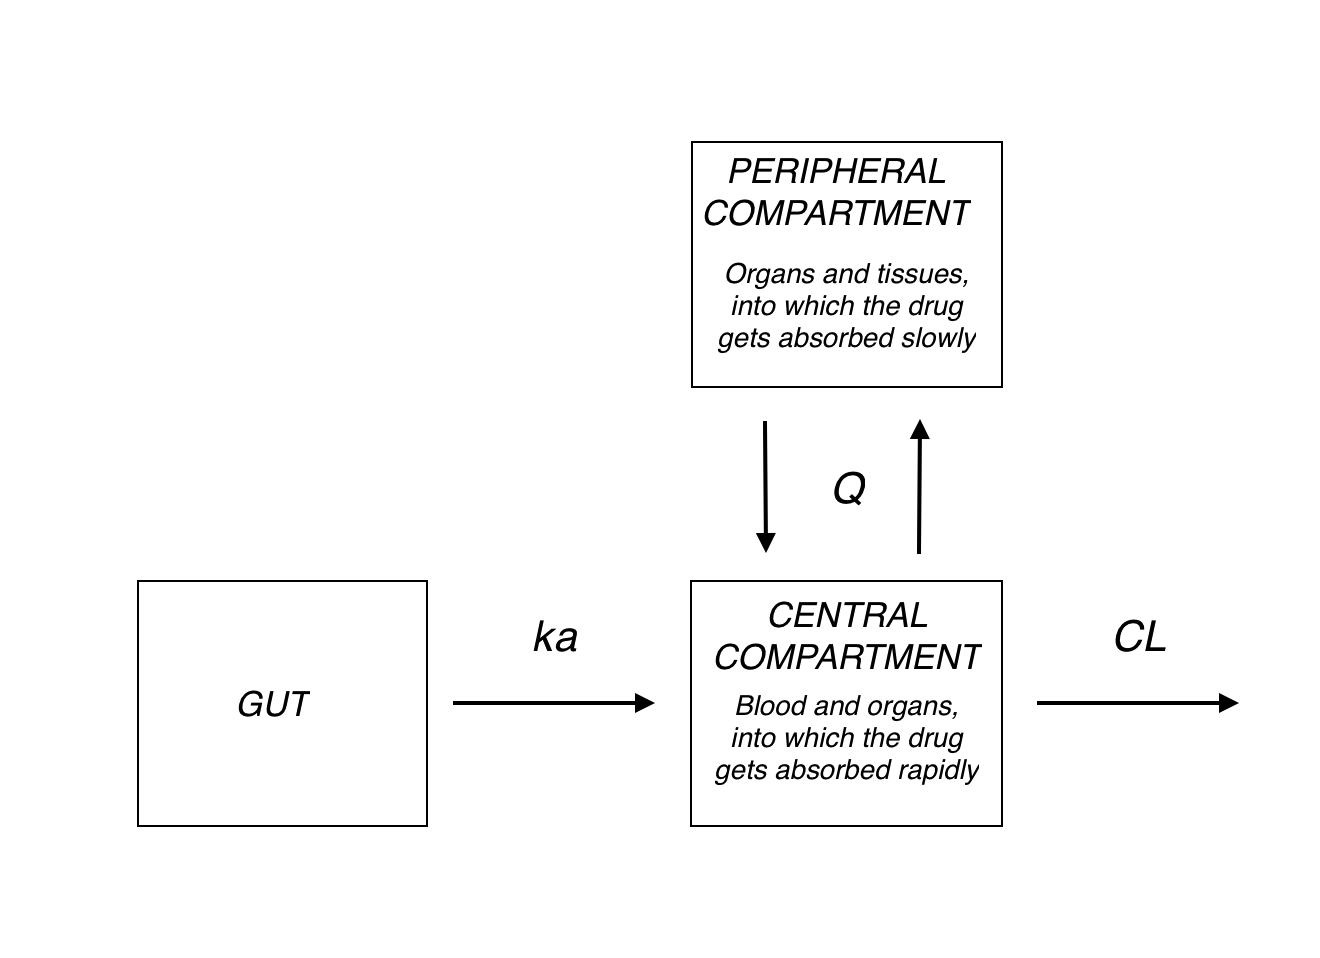
\includegraphics[width=4in]{../figures/TwoCptNice.png}
  \end{center}
 
\end{frame}

\begin{frame}
  \frametitle{Two compartment model}
  
  \begin{eqnarray*}
  \begin{aligned}
  y_\mathrm{gut}' &= -k_a y_\mathrm{gut} \\
  y_\mathrm{cent}' &= k_a y_\mathrm{gut} - \left(\frac{CL}{V_\mathrm{cent}} + \frac{Q}{V_\mathrm{cent}} \right) y_\mathrm{cent} +  \frac{Q}{V_\mathrm{peri}} y_\mathrm{peri} \\
  y_\mathrm{peri}' &= \frac{Q}{V_\mathrm{cent}} y_\mathrm{cent} - \frac{Q}{V_\mathrm{peri}} y_\mathrm{peri}
  \end{aligned}
  \label{eq:2Cpt}
\end{eqnarray*}

\end{frame}

\begin{frame}
  \frametitle{Example 2: Bone mineral density model from \cite{Peterson:2012}}
  \begin{center}
    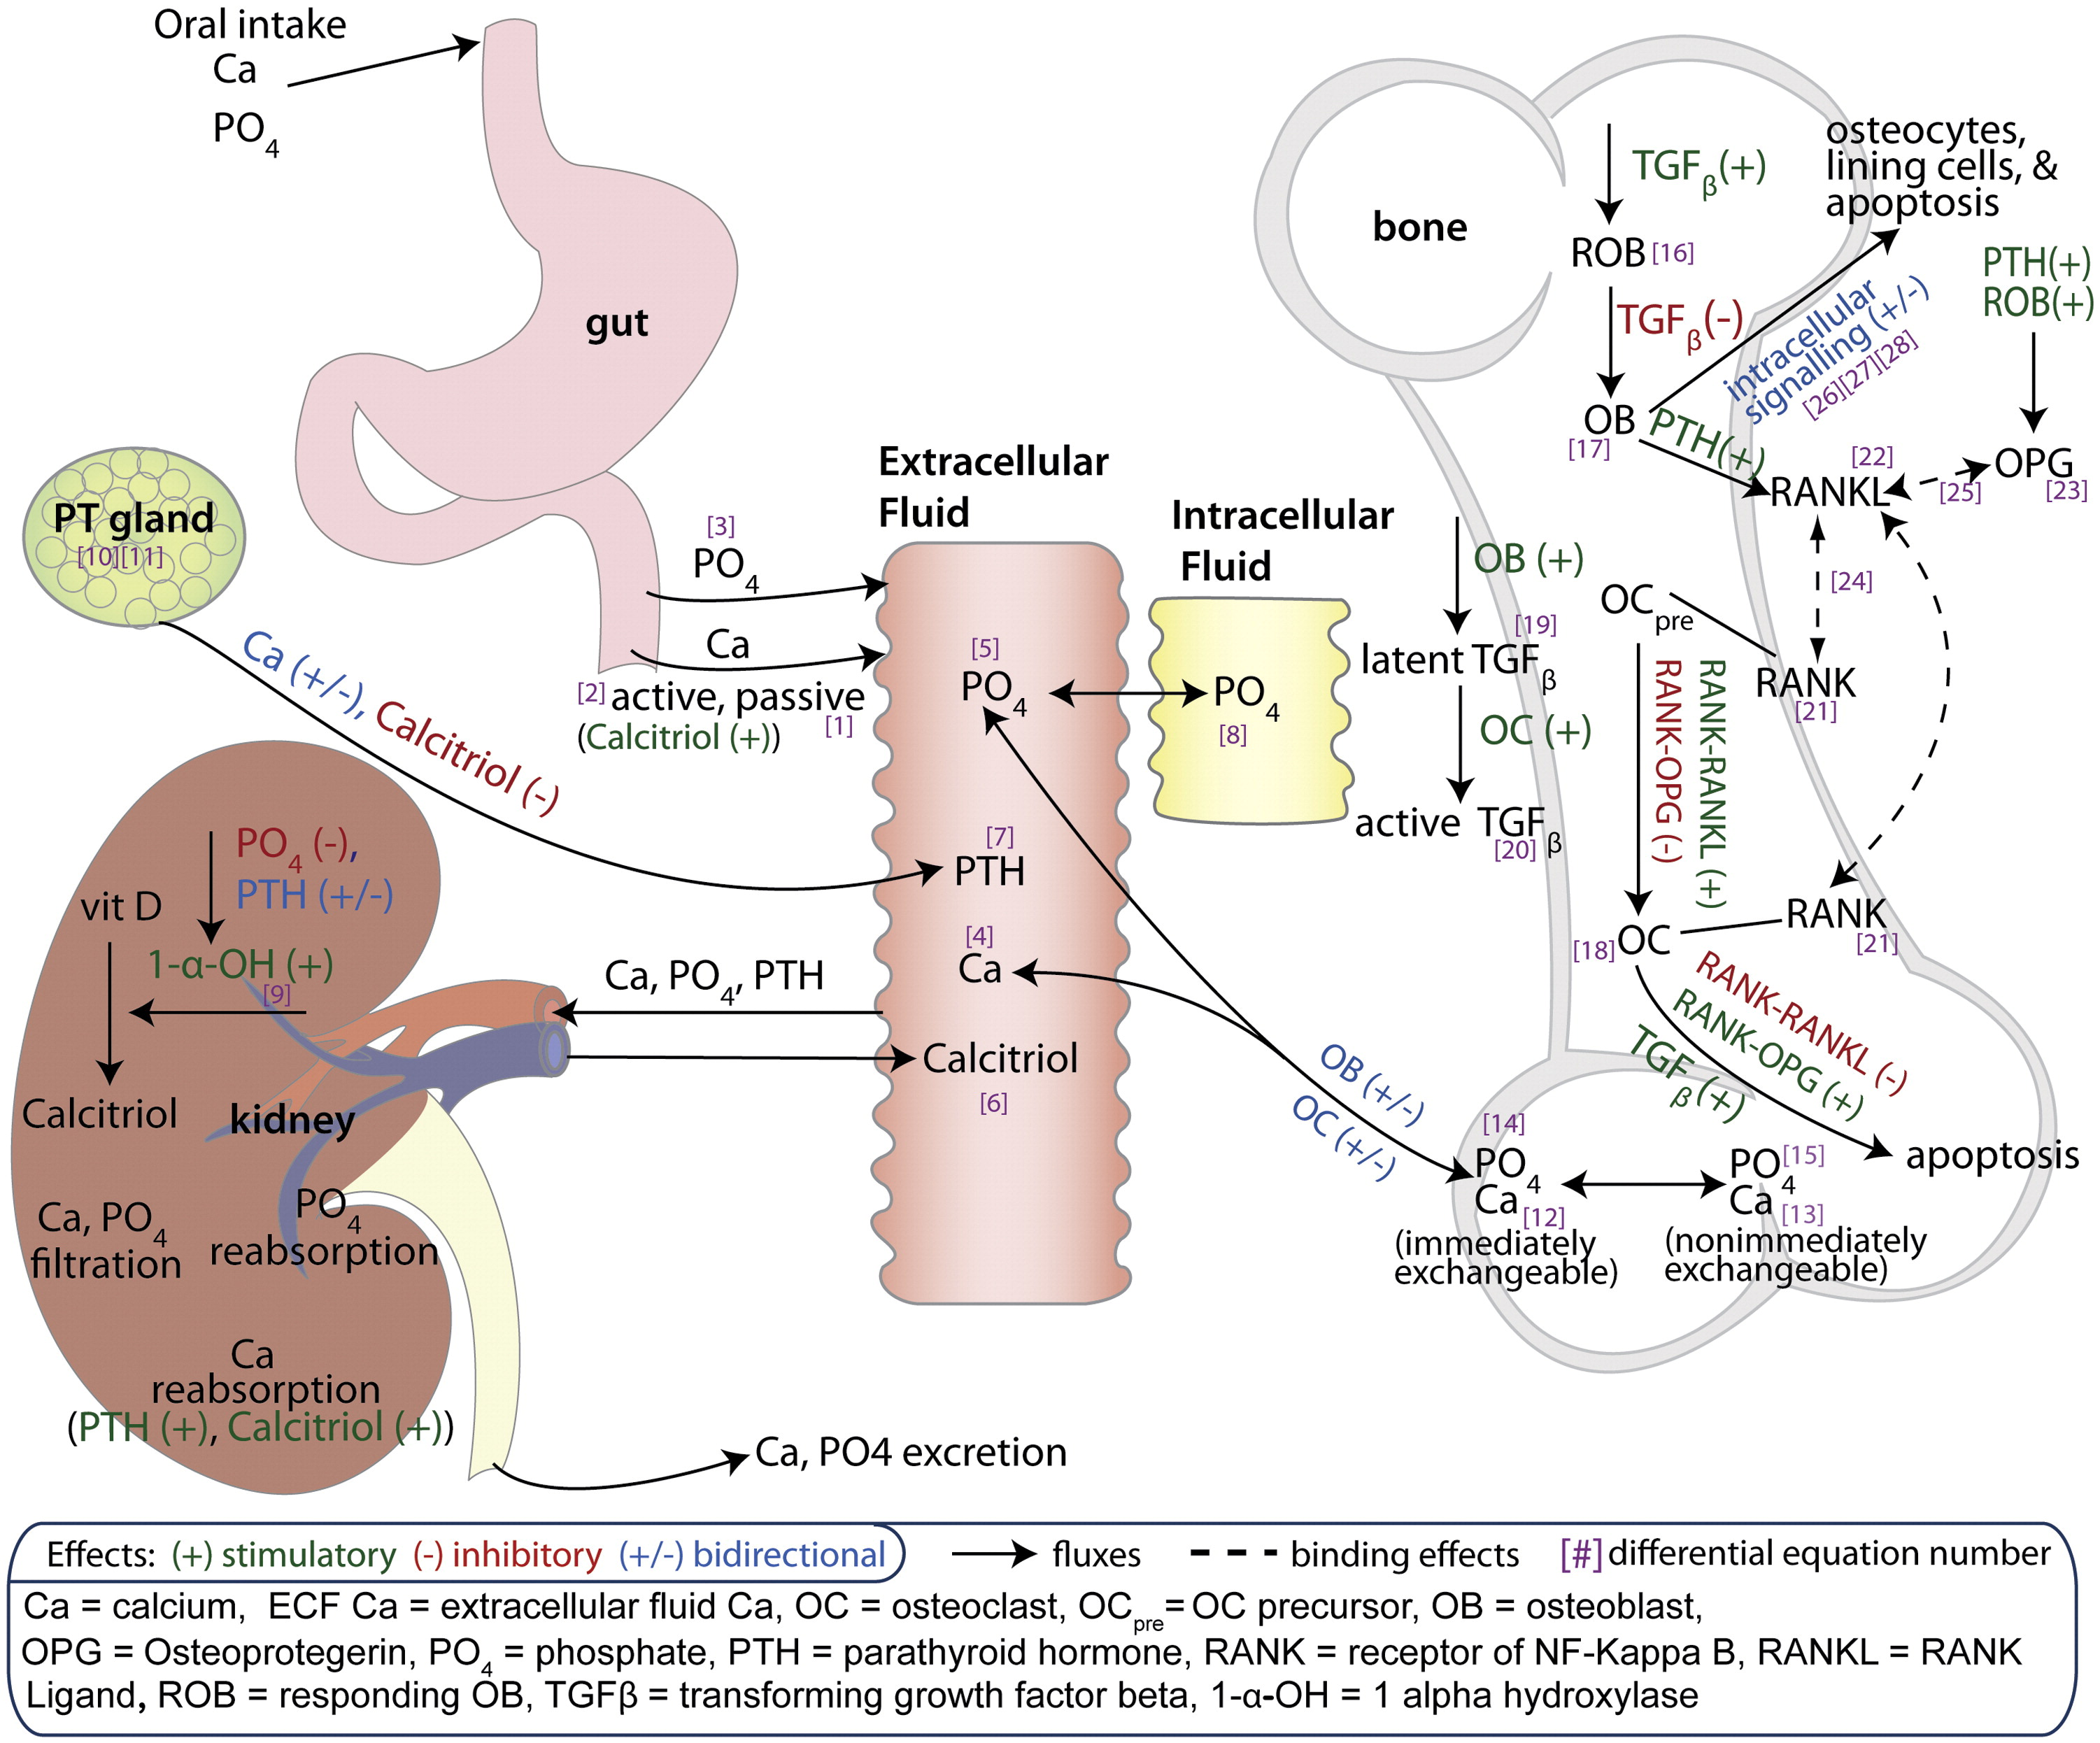
\includegraphics[width = 3in]{../figures/RiggsBoneModel.jpg}
  \end{center}

\end{frame}

\begin{frame}
    \frametitle{Two compartment model}
    
    Denote $\theta = \{CL, Q, VC, VP, K_a \}$, the ODE coefficients.
    Then
    $$ y' = f(y, t, \theta) $$
    
    Given an initial condition $y_0 = y(t_0)$, solving the above ODE gives us
    the \textcolor{MRGGreen}{\textit{natural evolution}} of the system at any given time point.

\end{frame}

\begin{frame}
  \frametitle{The event schedule}
  
  An event can be:
  \begin{itemize}
    \item \textcolor{MRGGreen}{Sate changer}: an (exterior) intervention that alters the state of the system;
    for example a bolus dosing or the beginning of an infusion.
    \item \textcolor{MRGGreen}{Observation}: a measurement of a quantity of interest at a certain time.
  \end{itemize}

\end{frame}

\begin{frame}
  \frametitle{Drug concentration in a patient's blood}
  
  \begin{center}
    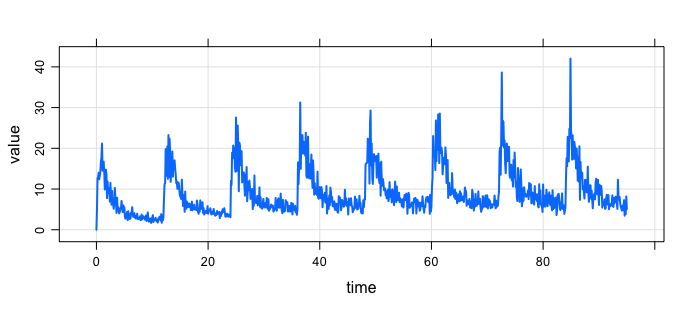
\includegraphics[width=3.5in]{../figures/multiple_doses.png}
  \end{center}

\end{frame}

\begin{frame}
  \frametitle{The event schedule}
  
  \begin{itemize}
    \item There is no general theory for the event schedule :(
    \item The modeling software NONMEM\textregistered \ proposes a convention for pharmacometrics,
    which we adopt in Torsten.
  \end{itemize}

\end{frame}

\begin{frame}
  
  Torsten offers additional built-in functions to simulate data from a compartment model.
  
  \begin{center}
    
\includegraphics[width=1.5in]{../torstenLogo.png}
  \end{center}
  
  Each Torsten function requires users to specify:
  \begin{itemize}
    \item a system of ODEs and a method to solve it.
    \item An event schedule.
  \end{itemize}

\end{frame}

\begin{frame}
  \frametitle{Torsten function}
  
  \texttt{
    pmx\_solve\_onecpt(time, amt, rate, ii, evid, \\ 
    \hspace{3.3cm} cmt, addl, ss, \\
     \hspace{3.3cm} theta, biovar, tlag)
   }
  
\end{frame}

\begin{frame}
  \frametitle{Torsten function}
  
  \texttt{
    pmx\_solve\_\textcolor{MRGGreen}{twocpt}(time, amt, rate, ii, evid, \\ 
    \hspace{3.3cm} cmt, addl, ss, \\
     \hspace{3.3cm} theta, biovar, tlag)
   }
   
   \ \\
   \begin{itemize}
     \item analytically solve the ODEs for the two cpt model. 
   \end{itemize}
  
\end{frame}

\begin{frame}
  \frametitle{Torsten function}
  
  \texttt{
    pmx\_solve\_twocpt(\textcolor{MRGGreen}{time, amt, rate, ii, evid, \\ 
    \hspace{3.3cm} cmt, addl, ss}, \\
     \hspace{3.3cm} theta, biovar, tlag)
   }
   
   \ \\
   \begin{itemize}
     \item the event schedule
   \end{itemize}

\end{frame}

\begin{frame}
  \frametitle{Torsten function}
  
  \texttt{
    pmx\_solve\_twocpt(time, amt, rate, ii, evid, \\ 
    \hspace{3.3cm} cmt, addl, ss, \\
     \hspace{3.3cm} \textcolor{MRGGreen}{theta}, biovar, tlag)
   }
   
   \ \\
   \begin{itemize}
     \item the ODE coefficients $\theta = \{CL, Q, VC, VP, ka \}$ 
   \end{itemize}
  
\end{frame}

\begin{frame}
  \frametitle{Torsten function}
  
  \texttt{
    pmx\_solve\_twocpt(time, amt, rate, ii, evid, \\ 
    \hspace{3.3cm} cmt, addl, ss, \\
     \hspace{3.3cm} theta, \textcolor{MRGGreen}{biovar, tlag})
   }
   
   \ \\
   \begin{itemize}
     \item bio-availibility fraction and lag times. 
   \end{itemize}
  
\end{frame}

\begin{frame}
  \frametitle{Example}
  Clinical trial:
  \begin{itemize}
    \item Single patient
    \item Bolus doses with 1200 mg, administered every 12 hours, for a total of 15 doses.
    \item Many observations for the first, second, and last doses.
    \item Additional observation every 12 hours.
  \end{itemize}

  \ \\ Note: the observation are plasma drug concentration measurement.

  \ \\ See \texttt{data/twoCpt.data.r}.
\end{frame}

\begin{frame}
  
  Model:
  \begin{itemize}
    \item two compartment model with first-order absorption
    \item prior information based on clinical trial conducted on a large population
    \item normal error for the plasma drug concentration measurement.
  \end{itemize}

\end{frame}

\begin{frame}
  Prior:
  \begin{eqnarray*}
    CL & \sim & \mathrm{logNormal}(\log 10, 0.25) \\
    Q & \sim & \mathrm{logNormal}(\log 15, 0.5) \\
    VC & \sim & \mathrm{logNormal}(\log 35, 0.25) \\
    VP & \sim & \mathrm{logNormal}(\log 105, 0.5) \\
    ka & \sim & \mathrm{logNormal}(\log 2.5, 1) \\
    \sigma^2 & \sim & \mathrm{half-Cauchy}(0, 1)
  \end{eqnarray*}
  
  Likelihood:
  \begin{eqnarray*}
    \log(cObs) & \sim & \mathrm{Normal}\left( \log \left(\frac{y_2}{VC} \right), \sigma^2 \right) 
  \end{eqnarray*}
  
   \textit{\textcolor{MRGGreen}{Exercise 1}: write and fit this model, 
   using \texttt{twoCptModel.r} and  \texttt{model/twoCptModel.stan}.}

\end{frame}

\begin{frame}

  \textit{\textcolor{MRGGreen}{Exercise 2}:
     Write a generated quantities block and do posterior predictive checks.}
\end{frame}

\begin{frame}
  \frametitle{Resources}

  \begin{itemize}
    \item Torsten repository: \url{https://github.com/metrumresearchgroup/Torsten}
    \item Torsten User manual (on GitHub and in the workshop folder).
  \end{itemize}
\end{frame}

\section{References}
\begin{frame}[allowframebreaks]{References}
\scriptsize
% \bibliographystyle{unsrt}
%\bibliographystyle{authoryear}
\bibliographystyle{apalike}
\bibliography{../ref}  
\end{frame}

\end{document}
